% arara: pdflatex: { synctex: yes }
% arara: makeindex: { style: ctuthesis }
% arara: bibtex

% The class takes all the key=value arguments that \ctusetup does,
% and a couple more: draft and oneside
\documentclass[twoside]{ctuthesis}
\usepackage{algorithmicx}
\usepackage{algpseudocode}
\usepackage{algorithm}
\algdef{SE}[DOWHILE]{Do}{doWhile}{\algorithmicdo}[1]{\algorithmicwhile\ #1}%


\ctusetup{
	preprint = \ctuverlog,
%	mainlanguage = english,
%	titlelanguage = czech,
	mainlanguage = english,
	otherlanguages = {slovak,english},
	title-czech = {Moje bakalářka se strašně, ale hrozně dlouhým předlouhým názvem},
	title-english = {My Favourite Thesis; Just the Title is Soooooooo Looooong},
	subtitle-czech = {Cesta do tajů kdovíčeho},
	subtitle-english = {Journey to the who-knows-what wondeland},
	doctype = B,
	faculty = F4,
	department-czech = {Katedra matematiky},
	department-english = {Department of Mathematics},
	author = {Matouš Pelikán},
	supervisor = {Prof. Krutoš Spravedlivý},
	supervisor-address = {Ústav X, \\ Uliční 5, \\ Praha 99},
	supervisor-specialist = {John Doe},
	fieldofstudy-english = {Mathematical Engineering},
	subfieldofstudy-english = {Mathematical Modelling},
	fieldofstudy-czech = {Matematické inženýrství},
	subfieldofstudy-czech = {Matematické modelování},
	keywords-czech = {slovo, klíč},
	keywords-english = {word, key},
	day = 10,
	month = 2,
	year = 2017,
	specification-file = {ctutest-zadani.pdf},
%	front-specification = true,
%	front-list-of-figures = false,
%	front-list-of-tables = false,
%	monochrome = true,
%	layout-short = true,
}

\ctuprocess

\addto\ctucaptionsczech{%
	\def\supervisorname{Vedoucí}%
	\def\subfieldofstudyname{Studijní program}%
}

\ctutemplateset{maketitle twocolumn default}{
	\begin{twocolumnfrontmatterpage}

		\ctutemplate{twocolumn.abstract.in.titlelanguage}
		\ctutemplate{twocolumn.abstract.in.secondlanguage}
		\ctutemplate{twocolumn.tableofcontents}
		\ctutemplate{twocolumn.listoffigures}
	\end{twocolumnfrontmatterpage}
}

% Theorem declarations, this is the reasonable default, anybody can do what they wish.
% If you prefer theorems in italics rather than slanted, use \theoremstyle{plainit}
\theoremstyle{plain}
\newtheorem{theorem}{Theorem}[chapter]
\newtheorem{corollary}[theorem]{Corollary}
\newtheorem{lemma}[theorem]{Lemma}
\newtheorem{proposition}[theorem]{Proposition}

\theoremstyle{definition}
\newtheorem{definition}[theorem]{Definition}
\newtheorem{example}[theorem]{Example}
\newtheorem{conjecture}[theorem]{Conjecture}

\theoremstyle{note}
\newtheorem*{remark*}{Remark}
\newtheorem{remark}[theorem]{Remark}

\setlength{\parskip}{0.5ex plus 0.2ex minus 0.2ex}






% Only for testing purposes
\listfiles
\usepackage[pagewise]{lineno}
\usepackage{lipsum,blindtext}
\usepackage{mathrsfs} % provides \mathscr used in the ridiculous examples

\begin{document}
	
\maketitle


\chapter{Introduction}


Combinatorial optimization problems are a class of challenging tasks that involve finding the best arrangement or combination of discrete elements from a large set of possibilities. These problems arise in various fields, such as logistics, scheduling, network design, and resource allocation. Examples of combinatorial optimization problems include the traveling salesman problem (TSP), the knapsack problem, or the graph coloring problem to name only a few. The complexity of these problems lies in the exponential growth of possible solutions as the problem size increases, making it computationally infeasible to search the entire solution space.

Metaheuristics have emerged as a powerful technique to face the computational challenges posed by complex combinatorial problems. Metaheuristics provide a flexible and robust framework for addressing optimization challenges by operating at a higher level of abstraction. These algorithms offer a unique approach to problem-solving by exploring large solution spaces efficiently and effectively. They are particularly well-suited for combinatorial optimization problems where traditional methods, such as linear programming, integer programming, etc., struggle due to the high-dimensional and non-linear nature of the search space.

Among many other, evolutionary algorithms (EAs) represent a powerful class of metaheuristics that have demonstrated remarkable effectiveness in solving combinatorial optimization problems. Inspired by the principles of natural evolution, these algorithms emulate the process of natural selection and adaptation to guide the search for optimal or near-optimal solutions. They typically work with a population of individuals, where each individual represents a possible solution to the problem at hand. On top of what EAs can offer, it is common practise to integrate local search techniques in order to enhance the performance. Local search focuses on exploring the neighborhood of a given solution to find better nearby solutions. By combining local search with evolutionary algorithms, the search process benefits from both global exploration and local exploitation, leading to improved solution quality and convergence.

An example of such evolutionary based algorithm is IREANN, introduced by Kubalík and Snížek in \cite{kubalik2014novel}. IREANN uses an indirect representation and a so-called nearest neighbor heuristic, which is a constructive procedure suited for routing problems. Both of these concepts used in IREANN are heavily exploited in this thesis. Local search heuristics might be incorporated to IREANN to yield even better performance.

However, given the nature of IREANN's indirect representation functionality, improvements made by local search heuristics would only affect the single individual whose neighborhood of solution space was searched. The information about local improvements can not be easily passed between other individuals in a population. 

The objective of this thesis is to propose an extension to the IREANN algorithm that enables the propagation of valuable information about high-quality features of individual solutions across the entire population during computation. This extension aims to ensure that the entire population can potentially benefit from the insights gained from individually discovered superior features, thereby enhancing the overall performance and optimization capabilities of the algorithm.

The principle of enhancing the algorithm si to incorporate a mechanism that during computation captures and retains information about the features that contibute the most to high-quality solutions. The mechanism involves periodically storing the relevant information which is subsequently used in the nearest neighbor heuristic, and serves as a proxy to information about distance. The whole algorithm was specifically designed to solve the Capacitated arc routing problem (CARP), which is more challenging than the famous TSP and introduces more constraints.

Several slight modifications of above mentioned approach have been implemented as a result of this thesis. The effects of proposed extension on solution quality were empirically verified by testing on standard available CARP benchmark datasets.

The thesis is structured as follows...(TODO)

\chapter{Problem definition}
The capacitated arc routing problem (CARP), firstly introduced by Golden and Wong \cite{golden1981capacitated}, is a subject in combinatorial optimization, commonly appearing in operations research and transportation logistics. In this chapter, we will provide a formal definition of the CARP, establish relevant terminology, and underline the basic properties that characterize this complex problem.

The Capacitated Arc Routing Problem (CARP) is a variant of the arc routing problem where a fleet of vehicles of uniform capacity is used to service a set of arcs or edges in a network. The fundamental challenge is to design the minimum cost set of routes such that each vehicle originates and terminates at a depot, each edge in the network requiring service is traversed by exactly one vehicle, and the total demand serviced by any vehicle does not exceed its capacity.

The problem is defined on a connected, undirected graph \emph{G} = (\emph{V, E}), where V is the set of vertices and E is the set of edges. Every edge \emph{e} $\in$ \emph{E} has a non-negative cost or length \emph{$ c_e $} and a non-negative demand for service \emph{$ d_e $}. The edges with positive demand make up the subset of the required edges \emph{$ E_R $}. In CARP, the graph is typically undirected, meaning that each edge can be traversed in either direction with equal cost. 
The demand \emph{$ d_e $} of an edge \emph{e} represents the quantity of some resource or service that must be delivered along that edge. Each vehicle has a maximum capacity Q and the total demand of all edges in its route cannot exceed this capacity.
Given a vehicle capacity \emph{Q}, the CARP consists
of finding a set of vehicle routes of minimum cost,
such that every required edge is serviced by exactly
one vehicle, each route starts and ends at a prespecified vertex \emph{$ v_0 $} $\in$ \emph{V} (the depot) and the total
demand serviced by a route does not exceed the
vehicle capacity \emph{Q}. Golden and Wong \cite{golden1981capacitated} show that the CARP is NP-hard. 


\chapter{Related work}
Capacitated Arc Routing Problems (CARP) are known to be NP-hard problems. Due to its complexity, it is possible to solve it exactly only for small-sized instances. Instances of larges size usually make use of heuristic, more specifically metaheuristic approaches.

This chapter gives an overview of known 

\section{Exact and lower bound methods}
Lower bound methods provide a tight lower bound on its optimal cost. Such a bound is helpful when evaluating larger CARP instances, where heuristic approach has to be employed, since solving them exactly would be computationally too demanding and not feasible at all. Thus, achieving a solution which is close to a lower bound might be a good measure of quality for heuristic algorithms.
A simplified integer linear model was proposed by Belenguer and Benavent \cite{BELENGUER2003705}. The sparse formulation used does not lead to a valid CARP solutions, but presents very tight lower bounds for the problem. Only one integer is used for each edge, which results in not being able to say which vehicles service which edges.

First possible way of solving CARP is based on transforming the problem into a node routing problem and then using existing VRP methods to solve it. Quality of the solution depends on how well, meaning how compact such a transformation can get. The goal is for the dimension to not increase drastically.
First transformation of its kind was introduced by Pearn, Assad and Golden \cite{PEARN1987285} which reduced the CARP problem into CVRP problem, but was regarded as unpractical, since the transformed CVRP problem had a graph with 3e + 1 vertices, where e is the number of required edges in CARP. Similar transformation was then proposed by Longo, Aragao and Uchoa \cite{LONGO20061823}, which further reduced the number of vertices to 2e + 1. Combined with a branch-and-cut-and-price algorithm, they observed effective results, solving all gdb instances for the first time and finding new optimum for val files and two for egl files.
More recently, a compact transformation was introduced recently by Les Foulds et al. \cite{foulds2015compact} where the number of nodes is at most larger only by one than the number of edges. Again, an adapted version of branch-and-cut-and-price algorithm for CVRPs was used to obtain the results. The authors managed to solve all of the instances from the gdb dataset, however some instances in the larger dataset egl were not solved satisfactorily.

As mentioned by Bode and Irnich \cite{bode2012cut}, converting arc routing problems into node routing ones has significant drawbacks, which are models with inherent symmetry, dense underlying networks or models with huge number of vertices. Therefore, it is worth considering specialized CARP methods to address these issues. 
Specialized exact algorithms for CARP often involve solving integer programs using branch-and-cut or branch-and-bound combined with column generation. Branch-and-cut uses a cutting plane approach, in which inequalities are added to the optimization problem.  By adding these cuts, the feasible region of the subproblems can be further restricted, which can help the algorithm find the optimal solution more efficiently. Column generation, on the other hand, involves iteratively generating and adding columns (variables) to the problem's constraint matrix until an optimal solution is found. Mentioned algorithms are used in \cite{bode2012cut}, \cite{bartolini2013improved} to solve instances with up to 190 nodes to optimality. Instances with number of nodes greater than 200 remain unsolved by exact approaches. 

\section{Heuristics}
Heuristics algorithms are approximate methods that are used to quickly find a solution to an optimization problem that is likely to be close to the optimal solution. They are typically used when the exact optimization problem is too computationally expensive to solve in a reasonable amount of time, which is the case for solving larger instances of the CARP. The main focus will be on meta-heuristics, which represent more general techniques applicable to wide range of optimization problems.

One of the most famous algorithms for solving CARP is a tabu search algorithm called CARPET proposed by Hertz, Laporte and Mitaz \cite{hertz2000tabu}. In CARPET, a solution in represented by a set of nodes representing all traversed edges. Solutions violating vehicle capacity are accepted but penalized. The search process in a tabu search is guided by the tabu rules, which specify which moves are allowed and which are "tabu" (forbidden) at each step. Number of improvement procedures which are used in the search process are presented in CARPET (Shorten, Drop, Add, Paste, Cut, Switch and Postopt).

Subsequently, Hertz and Mittaz in \cite{hertz2001variable} applied a new algorithm to solve the CARP, which is the Variable Neighborhood Descent algorithm (VND). It replaces the framework of the tabu search with the framework of the variable neighborhood search and achieves slightly better solutions. It involves exploring a sequence of neighborhoods around the current solution. Several descents with different neighborhoods are performed until a local optimum for all considered neighborhoods is reached. However successful the solutions, the encoding used by CARPET and VND leads to intricate improving procedure, thus potentially making the search space vast.

Lacomme, Prins and Ramdane-Ch{\'e}rif \cite{lacomme2001genetic} proposed a memetic algorithm (MA), a genetic algorithm hybridized with a local search). Genetic part of the algorithm is inspired by the process of natural evolution and use techniques such as selection, crossover, and mutation to search for the optimal solution to a problem. Based on this evaluation, the algorithm selects the fittest individuals to survive and reproduce, and combines their genetic material through crossover to create new offspring. Mutation is then used to introduce random changes to the genetic material of the offspring, in order to explore a wider range of potential solutions. MA uses a more compact and natural encoding. Each edge is represented by only two indices, one for each direction. A route can then be defined by a list of such indices. Two consecutive edges in a route are connected by implicit shortest paths, which can be computed in advance. This encoding scheme is very useful when only fraction of edges are required and has been used in almost all metaheuristics published after CARPET and VND. MA achieves is more successful on the standard testing sets than CARPET, while also being twice as fast.

Are recent tabu search algorithm for solving a modified version of the original CARP problem was recently proposed in \cite{lai2018forest}. They consider split-delivery CARP (SDCARP), which generalizes conventional CARP by allowing an arc to be serviced by more than one vehicle. Forest-based tabu search utilizing forest-based neighborhood operators is used in this approach.

A similar memetic algorithm to (MA) with extended neighborhood search (MAENS) was proposed in \cite{tang2009memetic}. This work proposed a novel local search operator, which is capable of searching using large step sizes and is less likely to become trapped in locally optimal solutions.

To tackle the largest CARP benchmark instances, Mei, Tang and Yao \cite{mei2013decomposing} present a mechanism called Random Route Grouping (RRG) designed to decompose the large-scale CARP (LSCARP). RRG is combined with a cooperative co-evolution (CC) model to give yield impressive result on large datasets. The cooperative co-evolution framework is a natural way to implement divide-and-conquer strategy. Generally, CC is a type of evolutionary algorithm that involves the simultaneous evolution of multiple subpopulations, or "species," that are interdependent and work together to find a solution to a problem. A bit later, authors of \cite{mei2014variable} improve on the decomposition procedure by incorporating information about the quality of the best solution found in the search.

Another group of possible meta-heuristic approaches are ant-colony algorithms, which are inspired by the behaviour of ant colonies. A set of artificial ants is initialized at selected locations of the network, the network is then explored by the ants which are combining local information (the cost of the arc connecting the current node to the next one), with the global information (pheromone levels on the arcs). Pheromone levels store the information about the quality of the solutions found so far. Ants deposit pheromones on the arcs as they traverse, which influences the behaviour of other ants. 
Tirkolaee et al. \cite{TIRKOLAEE2019457} introduce an ant colony based metaheuristic with some modifications. They use a modified version of the Ant Colony Optimization algorithm derived from Ant System called Max-Min Ant System (MMAS). MMAS was firstly presented by Stützle and Hoos in \cite{stutzle2000max}, their main contribution was the introduction of upper and lower bounds for the value of the pheromones which avoids stagnation of the search. \cite{TIRKOLAEE2019457} further improves the performance of MMAS by utilizing a mechanism called Pheromone Trial Smoothing (PTS), which results in preventing premature convergence, avoiding local optima and increasing efficient search space.

In \cite{martinez2011b}, a biased random key genetic algorithm is combined with a local search. Optimal or near optimal solutions were obtained while achieving small computation times during testing on sets of CARP benchmark instances. Classical local search methods which “fine-tune” its solutions are used to potentially find better ones. Local search might be applied in different ways. One is to pass the best solution found by RKGA to a local search algorithm to be further optimized, another possibility is to use local search as a mutation operator within RKGA.

Open CARP is a variant of the original CARP problem which releases the constraint which states that tours must begin and end at a depot, which means that the tours in this variant do not have form cycles. A recent work of \cite{arakaki2018hybrid} deals with the open CARP by introducing a Hybrid genetic algorithm, whose main features is standard genetic algorithm combined with local search and feasibilization procedure which is responsible for obtaining a feasible solution from chromosome. Feasibilization proved to have substantial role on performance. It also includes a population restart which avoids premature convergence of the population, which happens when the genetic diversity is low and only small are of the search space is being explored.

In some cases, the demand for a product or service may be uncertain or subject to random fluctuations. Such behaviour is modeled by one of the most recently studied variant of the CARP problem, the Uncertain CARP (UCARP). It was proposed to better reflect reality. In UCARP, the travel cost between vertices in the graph and demand of tasks is unknown in advance, and is revealed during the process of executing the services. In this case, a preplanned solution may become worse or even infeasible. Authors of \cite{wang2021genetic} propose a novel genetic programming approach, which simplifies the routing policies during the evolutionary process using a niching technique, which leads to a more interpretable policies. Niching is a technique used to preserve diversity among populations of solutions. It avoids aforementioned premature convergence, where the algorithm would get stuck in a local optimum. Instead of having a single population of solutions that all evolve together, niching involves dividing the population into subpopulations, or niches. These niches contain solutions that are similar to each other, but distinct from those in other niches. This way, the search space is expanded, increasing the chances of finding the best solution.


\chapter{Preliminaries}


\section{Overview of Evolutionary Algorithms}

Evolutionary Algorithms (EAs) are a diverse family of optimization techniques rooted in the principles of biological evolution. Mirroring nature's underlying processes, they use mechanisms inspired by natural selection and genetics to solve complex search and optimization problems. The general approach of EAs is to maintain a population of candidate solutions for the problem at hand and to iteratively improve this population over time. They are characterized by their population-based search approach, their utilization of stochastic processes, and their capability of maintaining and exploring a diversity of solutions. This provides an inherent robustness, allowing for a versatile exploration of the search space, and makes EAs well-suited for a wide range of problems, including those with large and intricate search spaces, non-linear relationships, or poorly understood fitness landscapes.

The main operators utilized within EAs are selection, crossover (or recombination), and mutation, which emulate the mechanisms of survival of the fittest, mating, and random genetic mutation respectively.

While all EAs share these commonalities, different types of EAs have emerged, fine-tuning these concepts to particular problem types or application areas. Each type has its unique features and specializations, with notable examples including Genetic Algorithms, Genetic Programming, Differential Evolution, Evolution Strategies, and Evolutionary Programming. These will be discussed in further detail below.

\section{Genetic Algorithms}

Genetic Algorithms (GAs) constitute a significant branch of EAs, with a strong emphasis on the mechanisms of natural selection and genetics. Taking inspiration from Charles Darwin's theory of natural evolution, GAs maintain a population of candidate solutions that evolve over generations.

Each individual solution in a GA is characterized by a set of parameters or variables, encoded in a data structure analogous to a chromosome. These chromosomes can be binary strings, real-valued vectors, or other appropriate structures depending on the specific problem being addressed.

The fitness of each individual is assessed using an objective function specific to the problem, similar to how an individual organism's fitness for survival might be measured in nature. This objective function acts as the primary evaluator and driver for the progression of solutions, pushing the evolution process towards optimal or near-optimal solutions.

GA operates using three main genetic operators:
\begin{itemize}
	\item Selection: This operator mimics the survival of the fittest principle. It selects the individuals with higher fitness values to pass their genes to the next generation.
	\item Crossover (or Recombination): It emulates the genetic recombination observed in nature, where offspring inherit genetic information from their parents. In GA, it is a method to create new candidate solutions by combining parts of the 'chromosomes' of two or more selected individuals from the current population.
	\item Mutation: This operator introduces random modifications in the chromosome of individuals, promoting genetic diversity and enabling the exploration of new areas of the search space.
\end{itemize}

While GAs are a part of the broader EA family, their distinctive feature lies in their particular implementation of the evolutionary principles. The concrete representation of solutions as chromosomes, the clear distinction of generations, and the straightforward usage of genetic operators make GAs a robust and versatile tool for a wide array of optimization problems.

\section{Evolutionary algorithms}

Evolutionary algorithms are population-based metaheuristics that are inspired by the process of natural selection. They are used to generate solutions to optimization and search problems by mimicking the process of biological evolution. Evolutionary algorithms typically involve the use of a population of candidate solutions, which are evolved over time through the application of genetic operators such as selection, crossover (recombination), and mutation. These operators are applied in a stochastic manner, allowing the population of solutions to explore different regions of the search space.

The basic idea behind evolutionary algorithms is to start with an initial population of solutions, and then repeatedly apply genetic operators to generate new generations of solutions. The solutions are typically represented as binary strings, real-valued vectors, or other data structures, depending on the specific problem being solved. The genetic operators are designed to mimic the processes of natural selection and genetic variation that occur in biological populations. For example, selection is used to select the most fit individuals from the current population, which are then used to generate the next generation. Crossover (recombination) is used to combine the genetic material of two parents to create a new offspring, while mutation is used to introduce small random changes into the genetic material.

The main advantage of evolutionary algorithms is their ability to explore large and complex search spaces, even when the fitness function is poorly understood or highly nonlinear. They are also highly robust, and can often find near-optimal solutions even when the initial population is poorly chosen. However, they can also be computationally intensive and may require a large number of function evaluations to converge.

The whole family of evolutionary optimization algorithms is referred to as evolutionary computation (EC) algorithms. In the evolutionary computation domain, the following algorithms are worth mentioning: the genetic algorithm, genetic programming, differential evolution, evolution strategy, and evolutionary programming. Each of these techniques has many different varieties and is used in many different industrial applications.

\section{Genetic algorithms}
The genetic algorithm is one of the oldest and most known optimization techniques, which are based on nature. In the GA, the search for solution space imitates the natural process which takes place in the environment, and the Darwinian theory of species evolution is taken into consideration. In GAs, we have a population of individuals. Each individual, characterized by a set of parameters called a chromosome, represents a potential solution to the problem. The problem being solved is defined by the objective function. Depending on how good the individual is according to the objective function, the value which represents its quality is attributed to it. This value is called the fitness of the individual, and it is its main evaluating factor. Individuals with better fitness values are more likely to be selected to the new generation of the population. In genetic algorithms, we usually have three operators: selection (a new population of individuals is created based on the fitness values of individuals from the previous generation), crossover (typically parts of individuals chromosomes are exchanged between two individuals selected to the crossover), and mutation (the values of particular genes are changed randomly)


\section{Genetic programming}
Genetic programming (GP) is specialized form of GA which operates on very specific types of solution, using modified genetic operators. The GP was developed by Koza \cite{koza1992genetic} in an attempt to find the way for the automatic generation of the program codes when the evalution criteria for their proper operation is known. Because the searched solution is a program, the evolved potential solutions are coded in the form of trees instead of linear chromosomes which are common for GAs. The genetic operators are specialized for working on trees, for example, crossover is exchanging the subtrees, mutation is changing nodes or leaves.

\section{Differential evolution}
The differential evolution (DE) is a type of evolutionary algorithm useful mainly for the function optimization in continuous search space. The principal version of the algorithm was discussed by Storn and Price \cite{storn1997differential} While its basic mechanism is similar to a GA, its mutation operator is quite different. It involves selecting two search points from the population, taking their vector difference, scaling by a constant, and then adding this to a third search, again sampled randomly from the population. The crossover operator of differential evolution recombines the mutated search point (the mutant vector) with another existing search point (the target vector), replacing it if the child solution (trial vector) has greater objective value.

\section{Evolution strategies}
The evolution strategies are different when compared to the genetic algorithms, mainly in the selection procedure. Genetic algorithms create new population by choosing individuals from the parent population based on their fitness value, keeping constant size of the population. In evolution strategies, a temporary population is created. It has different size then the parental population (depending on the parameters). Fitness value does not matter in this step, individuals in the temporary population undergo crossover and mutations. From such populations, a number of the best individuals are selected to the next generation of the population. Evolution strategies usually operate on the vectors of floating point numbers, whereas classical genetic algorithms operate on binary vectors.

\section{Evolution programming}
In evolutionary programming, the new population of individuals is created by mutating every mutating every individual from the parental population. The mutation is based on the random perturbation of the values of the particular genes of the mutated individual. The newly created and the parental population are the same sizes. The new generation is of the population is created using the ranking selection of the individuals from both, the parental and the mutated populations.

\section{Memetic Algorithms}
Memetic algorithms (MAs) represent an extension of the traditional genetic algorithms, which on top the genetic framework employ local search operators during the computation. They were invented by Moscato in \cite{moscato1989evolution}. MAs are described by Moscato as "a marriage between a population-based global search and the heuristic local search made by the individuals." The word "meme", which was the inspiration for the term memetic algorithms, denotes the idea of a unit of imitation. Moscato uses the analogy of martial arts to describe memes as those undecomposable movements, which when individually composed form a more complex movement. Put simply, memetic algorithms improve genetic algorithm, which rely almost entirely upon recombination mechanisms to improve solution quality, by combining them with some kind of local optimisation of each individual in population. 

\section{IREANN}
The foundation for the proposed extension in this thesis is based on the work of Kubalík and Snížek \cite{kubalik2014novel}. Their research introduces an evolutionary algorithm with indirect representation and extended nearest neighbor nonstructive procedure (IREANN), specifically designed for solving the Traveling Salesman Problem (TSP). The functionality and effectiveness of the IREANN algorithm in addressing the TSP are demonstrated in their study.

The proposed evolutionary algorithm uses an indirect representation as a sequence of required arcs (edges) which is called a priority list, where the order of arcs define the order in which the nodes will be inserted into an existing tour via extended nearest neighbor heuristic.
The optimal solution might be, depending on the nature of problem being solved and the instance, represented by many different priority lists, which is beneficial, because the optimum will be attracted by multiple different priority lists. On the other hand, the opposite might also happen, which is that the optimal solution would not be reachable by given representation because there exists no priority list that would represent it.

\subsection{Algorithm pseudocode}
 The extended nearest neighbor construction procedure:
\begin{algorithm}
 	\caption{CNNP for TSP}\label{alg:cap}
\begin{algorithmic}[1]
\State Initialize \emph{n} single node components \emph{$ start_i = i, end_i = i $} for \emph{$ i = 1, ..., n $}
\State $j \gets 1$
\Do
\State Take \emph{j}-th city, \emph{P[j]}, from the priority list \emph{P}
\State Identify component \emph{$ C_k $} to which city \emph{P[j]} belongs
\If{\emph{P[j] is either \emph{$ start_k $}} or \emph{$ end_k $} of \emph{$ C_k $}}
\State \emph{N} $\gets$ {\tt nearestNeighbor}(\emph{P[j]})
\State add edge (\emph{N}, \emph{P[j]})
\Else
\State \emph{$ N_1 $} $\gets$ {\tt nearestNeighbor}(\emph{$ start_k $})
\State \emph{$ N_2 $} $\gets$ {\tt nearestNeighbor}(\emph{$ end_k $})
\If{{\tt dist}(\emph{$ N_1, start_k $}) $\leq$ {\tt dist}(\emph{$ N_1, end_k $})}
\State add edge (\emph{$ N_1, start_k $})
\Else
\State add edge (\emph{$ N_2, end_k $})
\EndIf
\EndIf
\State \emph{j}++
\doWhile{$j \leq n$}

\end{algorithmic}
\end{algorithm}


\subsection{Indirect representation}
Crucial part of the algorithm, which is different from standard genetic algorithm approaches, is the indirect representation. It means that the chromosome does not represent the literal order of nodes in a route, but instead the chromosome is considered to be a priority list, where the order of nodes expresses an order in which the nodes will be inserted into a developed tour by means of the extended nearest neighbor heuristic.

For example, a priority
list {5, 2, 4, 1, 3} represents a solution that is constructed
through steps of application of the nearest neighbor heuristic
to the cities 5, 2, 4, 1 and 3, in this order.

\subsection{Extended nearest neighbor constructive procedure}
The procedure must be able to produce a valid tour of length \emph{n} for any input priority list.
The process starts with \emph{n} independent tour components. A component \emph{$ C_k $} is defined by its boundary cities {\emph{$ start_k, end_k $}}. Each city belongs to its own component at the beginning, \emph{$ start_i = i $} and \emph{$ end_i = i  $} for each city \emph{i} = 1, ..., \emph{n}

It iterates over the priority list and applies the nearest neighbor heuristic in the following fashion. At each iteration \emph{i}, an element of priority list \emph{$ P_i $} is processed. A component \emph{$ C_k $} is identified based on \emph{$ P_i $}, it may have one or multiple nodes already. If the selected \emph{$ P_i $} is one of the boundary nodes of \emph{$ C_k $}, then a city which is nearest to \emph{$ P_i $} is selected and added to the tour. Otherwise, the nearest neighbors of \emph{$ start_k $} and \emph{$ end_k $} of the component \emph{$ C_k $}, \emph{$ N_1 $} and \emph{$ N_2 $}, are found.
The shorter edge out of these two candidates, (\emph{$ N_1, start_k $}) and (\emph{$ N_2, end_k $}), is added to the constructed tour. 

In each step, two component are merged into a single one. The procedure repeats until there is only one component remaining, which represents the resulting route.

Figure \ref{fig:tsp} shows an illustration of the working of this procedure, which constructs a route from the priority list \emph{P} = \{ A, I, H, F, J, E, C, D, G, B \}. As you can see, \ref{fig:tsp} a) is the result of processing \{A, I, H, F\}, where nothing unexpected happens. Each time, a shortest link to node's neighbor is selected and added to a component, resulting in two components \{A, J, I\} and \{F, G, H\}. But when it comes to the node J, it is already a part of a component and is not a boundary node. That is why a nearest neighbor is looked for from nodes I and A. Link between I and H is shorter than the one from A to B, which is why the components are merged through the I and H edge. The final route depicted in \ref{fig:tsp} c) is obtained by applying the same rules for the rest of the priority list.
As already mentioned, there might be several priority lists which represent the same route in the end. In the case of this simple instance,  \{A, I, H, F, J, E, C, D, G, B\}, \{I, C, E, B, H, F, A, J, G, D\}, and \{F, A, C, H, I, E, D, B, G, J \} all lead to this same route. 

\subsection{Crossover, mutation, evolutionary algorithm}
The rest of the algorithm uses standard operators common to evolutionary approaches which are not particularly important for the CARP modification.


\begin{figure}
	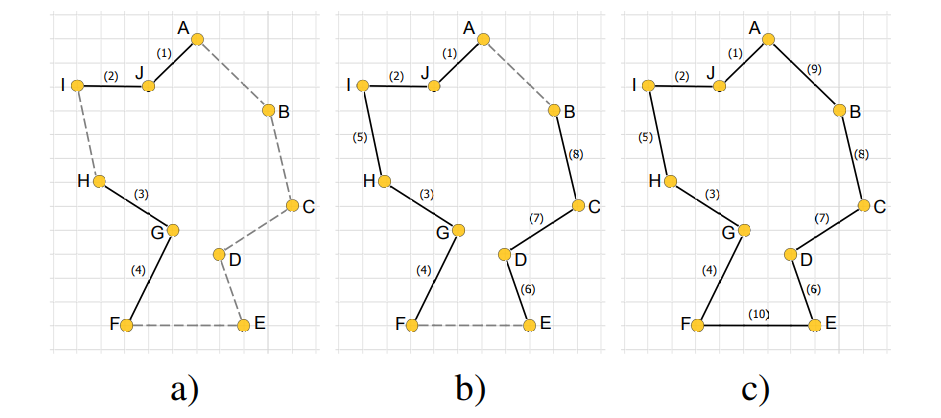
\includegraphics[width=\linewidth]{tspexample.png}
	\caption{Example of the extended nearest neighbor constructive
		procedure.}
	\label{fig:tsp}
\end{figure}


\section{IREANN modification to CARP}
We already defined the IREANN algorithm and its application of the Traveling salesman problem. In order to solve the Capacitated arc routing problem using similar approach, we need to develop multiple mechanisms specific to the CARP domain.

The biggest difference, obviously, is the fact that TSP deals with nodes, whereas CARP deals with edges. Therefore, the priority list for CARP modification of IREANN has to be a list of edges, more specifically those edges which are required. The constructive nearest neighbor procedure has to undergo several modifications. While searching for the fittest neighboring edge, we have to consider both ends for single edge route and those ends of edge which are not connected in multi-node routes.

One of the most crucial tasks is to develop a way of evaluating which neighbor of the so far developed route is the most suitable for extension, i.e. define a function which for every arc return a priority list of neighbors sorted by the aformentioned criterion. We absolutely need this functionality in order for the constructive nearest neighbor heuristic to work properly. For this purpose, we will draw some inspiration from \cite{5200351} and \cite{ULUSOY1985329}, which consider multiple rules for selecting the best neighboring edge, as well as the path scanning heuristic, a few traditional move operators used by the local search procedure along with the Merge-Split operator.

\subsection{Merge-Split operator}
In \cite{5200351}, the mentioned selection rules are used inside the Merge-Split operator, a local search procedure which aims to improve a given solution by modifying multiple routes of it. MS operator randomly selects \emph{p} routes from a given solution and merges them into an ordered list which contains all of the edges present in the \emph{p} routes that it previously selected. Then the path-scanning (PS) heuristics is used to construct a feasible set of routes. PS iteratively adds edges to the end of the current path (This is different to the IREANN approach, where we consider both ends of the current node for the selection) as long as they do satisfy the capacity constraints. If neighboring edge would satisfy the capacity constraints, then then the end of the route is connected to depot via shortest path. If more than one task satisfy the constraints, the aformentioned selection rules finally come to play: 1) maximize
the distance from the head of task to the depot; 2) minimize
the distance from the head of task to the depot; 3) maximize
the term \emph{dem}(t)/\emph{sc}(t), where \emph{dem}(t) and \emph{sc}(t) are demand
and serving cost of task t, respectively; 4) minimize the term
\emph{dem}(t)/\emph{sc}(t); 5) use rule 1) if the vehicle is less than halffull, otherwise use rule 2)
These 5 criteria are used to produce 5 different ordered lists of tasks, which are then passed to to Ulusoy's splitting procedure, defined in \cite{ULUSOY1985329}, which is an exact algorithm that finds the optimal way to split the ordered list into different routes. The best one out of these 5 candidates is chosen as the output of the MS operator. Major drawback of MS operator is its time complexity, which is considerably greater than the traditional local search operators.

\subsection{Traditional move operators for local search}
Some of the traditional, less computationally demanding operators for local search will also be utilized. We listed only the most fundamental move operators, but many others might be utilized, some of them are mention in \cite{BEULLENS2003629}.
\subsubsection{Single insertion}
This move operator works by taking an element from a current solution, and inserting it into a different position in the same solution. This creates a new solution that is a small variation of the original. 
\subsubsection{Double insertion}
Very similar to single insertion, double insertion takes two consecutive elements and inserts them elsewhere as opposed to only one element.
\subsubsection{Swap}
Similary to single insertion, two tasks are selected a their position is exchanged.
\subsubsection{2-opt}
2-opt tries to reconnect edges for single or double routes and looks for improvements in the objective cost function. Again it selects the one with which reconnects edges that result in the best value of objective function.

\section{IREANN extensions}
The work is to be extended with a mechanism that identifies high-level solution components on the fly during the evolutionary process and uses them as new elements that can be used in the priority lists. A considerable challenge is posed when considering which parts of the priority lists are most valuable and should be considered as one indivisible part. The algorithm looks for similar patterns in population of candidates among the individuals with the best fitness score and them treats those parts the same way as it treats individual edges. Improvements in performance are expected as a result of employing this approach. Optimal size of such chunks has to be determined.	

\chapter{Thesis}
\section{Memetic Algorithms}
Memetic algorithms (MAs) represent an extension of the traditional genetic algorithms, which on top the genetic framework employ local search operators during the computation. They were invented by Moscato in \cite{moscato1989evolution}. MAs are described by Moscato as "a marriage between a population-based global search and the heuristic local search made by the individuals." The word "meme", which was the inspiration for the term memetic algorithms, denotes the idea of a unit of imitation. Moscato uses the analogy of martial arts to describe memes as those undecomposable movements, which when individually composed form a more complex movement. Put simply, memetic algorithms improve genetic algorithm, which rely almost entirely upon recombination mechanisms to improve solution quality, by combining them with some kind of local optimisation of each individual in population. 

\section{Proposed approach}
To tackle the task of the capacitated arc routing problem (CARP), we will implement an algorithm which falls into the category of memetic algorithms, introduced in section [...]. Standard memetic approach will be enhanced with a mechanism which, at given generation, looks at the population of candidate solutions and identifies traits that lead to high-quality solutions amongst the best individuals, we call this 

\subsection{Carp modifications}

\subsubsection{Constructive procedure}
In section [...], constructive nearest neighbor procedure was introduced and its functionality was demonstrated on the travelling salesman problem. However, applying the same concept of CNNP to the capacitated arc routing problem inevitably calls for a couple of modifications to suit its need and constraints.
	
\begin{algorithm}
\caption{CNNP for CARP}\label{alg:cap}
\begin{algorithmic}[1]
	\State Initialize \emph{n} single edge components \emph{$ start_i = i, end_i = i $} for \emph{$ i = 1, ..., n $}
	\State $j \gets 1$
	\While{$j \leq n$}
	\State Take \emph{j}-th edge, \emph{P[j]}, from the priority list \emph{P}
	\State Identify component \emph{$ C_k $} to which edge \emph{P[j]} belongs
	
	TODO
	
	\State \emph{j}++
	\EndWhile
	
	
\end{algorithmic}
\end{algorithm}


 

\subsubsection{Solution feasibility}
Because of the nature of the capacitated arc routing problem, the challenge of solution feasibility arises. After the evaluation of given individual using the nearest neighbor constructive procedure, it is possible the resulting set of routes violates the constraint of maximum vehicle used. Such problem would not come up if the goal was to solve the Travelling salesman problem using similar heuristic to NNCP, but for the CARP which defines the maximum vehicle contraint, solutions violating this constraint are not acceptable. 

Another constraint is the maximum capacity of each vehicle, meaning that the sum of demands of each required edge must not exceed the defined limit, which is same for the whole fleet. The solutions however can not possibly violate this constraint thanks to the way the routes are constructed via the CNNP. (See section [...]) CNNP does not allow a route to be extended with another one which would result in such violation. That results in only the maximum vehicle count being vulnerable to violation, not the maximum capacity constraint which is always satisfied with this approach.

One idea would be to leave every infeasible solution out of the population of candidate solutions and not consider them at all. However, this approach would cause a lot of trouble, because in order to create the initial population, chromosomes of individuals in the first generation are set arbitrarily. Those chromosomes with randomly ordered genes are very unlikely to generate a valid solution in terms of the number of vehicles used, which would make it really hard to get an initial generation of only individuals with feasible solutions.

Instead, individuals representing infeasible solutions are allowed to exist in the population, but we need a way of telling which infeasible solutions are better than others in order to converge to a population with feasible individuals. 

That is where the fitness evaluation of each individuals comes into play.

That is why we need a way of determining which one of two infeasible individuals is better some sense, although neither of them is acceptable as a valid solution to the problem.

\subsubsection{Fitness function}
For the reasons stated in the previous section [Solution feasibility], we have to come with a mechanism which incentivizes the population to converge to a state where there are only individuals with valid number of vehicles. This will be done through designing a custom fitness evaluation.

Unfortunately, the fitness score of each individual can not simply be the total cost of its routes, because of the possibility of a situation where a solution with lower cost and a number of vehicles over the limit would be considered more fit than a solution with satisfactory number of vehicles and a greater cost, which is obviously an undesirable behaviour. On a more abstract note, optimisation of two variables at the same time is not possible, so the fitness evaluation will prioritize driving the vehicle count down first, and after that optimize the total routes cost when a satisfactory vehicle count has been reached.

This desired functionality is achieved by abandoning the idea of a single number determining the fitness of an individual, but instead implementing a custom comparator, which is used to sort the population. At the end that is what the fitness function is for, to tell how good the solutions are with respect to each other so that during the selection phase (details in section [...]), the right individuals according to selection rules and picked to be mated with each other. 

Comparator is a method which takes two individuals as input and decides which one of them is more fit according to criteria mentioned above. Several options might occur:
\begin{itemize}
	\item Vehicle count of both individuals is greater than the limit, then the one with lower vehicle count is deemed more fit. The cost is the deciding factor only when the vehicle counts are equal.
	\item First individual has satisfactory vehicle count, the other has not. In this case, the first individual is preferred no matter the cost of their solution.
	\item Both vehicle counts are less or equal than the limit, then the individual with lower cost is preferred.
\end{itemize}


\subsection{Genetic algorithm}

\subsection{Selection}
\subsection{Crossover}
\subsection{Mutation}
\subsection{Local Search}

\section{Analysis}



\bibliographystyle{amsalpha}
\bibliography{references}


\end{document}